
\section{Introduction}

\href{http://www.reana.io/}{The REANA (REusable ANAlysis) platform}\cite{reana_paper} is a reproducible and reusable data analysis platform allowing researchers to specify computational workflow steps in several declarative languages (such as \href{https://www.commonwl.org/}{CWL} \cite{cwl_source} or \href{https://yadage.readthedocs.io/en/latest/}{Yadage} \cite{yadage_source}) to run their data analysis pipelines on containerised compute clouds, using different compute backends (such as \href{https://kubernetes.io/}{Kubernetes} and \href{https://research.cs.wisc.edu/htcondor/description.html}{HTCondor}). The computational workflows associated to research data analyses can be represented in the form of a Directed Acyclic Graphs (DAG) that topologically order the analysis steps and define their dependencies. The DAG workflows may consist of running several tens of thousands of computational tasks. The platform was developed with data analysis reproducibility and reusability in mind. \cite{openisnotenough_paper}


\section{Reusable Analysis Examples}

To support the community to adopt reproducible science practices in their analyses, \href{http://www.reanahub.io/#examples}{several REANA examples} have been created, covering a wide range of use cases. Their purpose is to demonstrate the usage of REANA in the context of high energy particle physics data analysis carried out at the European Organization for Nuclear Research (CERN), using software specific to each collaboration/experiment. The workflow to create these examples is illustrated in Fig. \ref{fig:workflow_creation_schema}.


\begin{figure}[H]
    \centering
    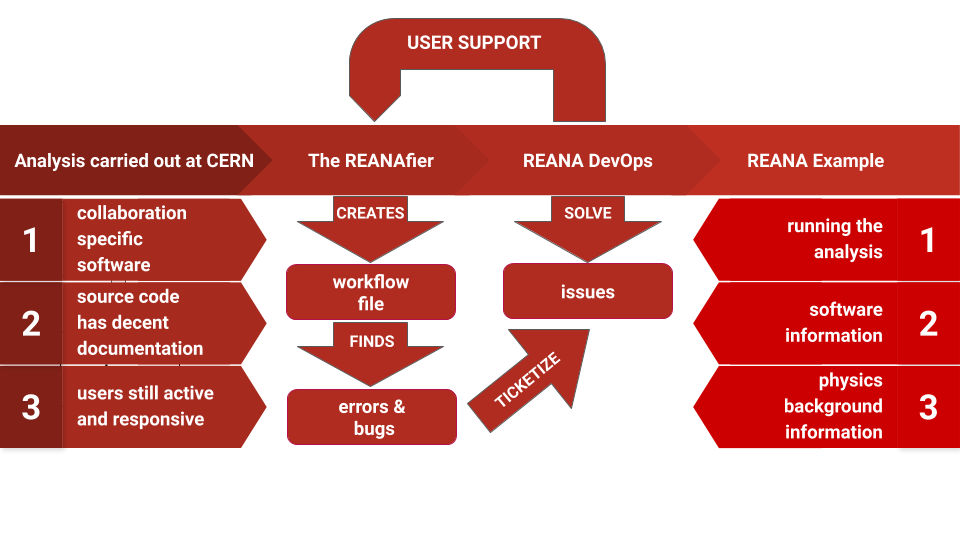
\includegraphics[width=0.8\textwidth]{figures/workflow_creation_schema.png}\\
    \caption{Typical workflow to create REANA examples from existing analysis carried out at CERN. As a first result of this Summer Project, the user experience has been vastly improved by adding new functionalities to REANA.}
    \label{fig:workflow_creation_schema}
\end{figure}


\subsection{ALICE Transverse Momentum $P_t$ Analysis Example}
\vspace{-1em}
\textit{The CERN Open Data Platform}\\
CERN has embarked the initiative to openly publish data from LHC experiments as open data to the public.\cite{COD-announcement}
"\href{http://opendata.cern.ch/}{The CERN Open Data portal} is the access point to a growing range of data produced through the research performed at CERN. It disseminates the preserved output from various research activities, including collision and simulated datasets, with accompanying software and documentation, which is needed to understand and analyse the data being shared.

\justify
The portal adheres to established global standards in Data Preservation and Open Science: the products are shared under open licenses; they are issued with a digital object identifier (DOI) to make them citable objects in the scientific discourse."\cite{COD-about} Moreover, they adhere to the FAIR Guiding
Principles for scientific data
management and stewardship. \cite{FAIR-principles}


\begin{figure}[H]
    \centering
    \begin{minipage}[H]{0.49\textwidth}
However, there is no explicit guarantee that any analysis code published online is actually working several years after it was originially published, if there is no continuous integration tool that checks it (\href{https://github.com/orgs/reanahub/projects/4}{GitLab integration} has been another Summer Project). Therefore, we wanted to test whether the ALICE open data example analysis can be actually reproduced using the information provided on the portal at the time of its publishing.\\

\vspace{1em}

\href{https://github.com/reanahub/reana-demo-alice-pt-analysis}{A new REANA example} has been set up using a material published by the \href{http://aliceinfo.cern.ch/Public/Welcome.html}{ALICE collaboration}, namely: a simple transverse momentum $P_t$  \href{http://opendata.cern.ch/record/1200}{analysis script} using any of the \href{http://opendata.cern.ch/search?page=1&size=20&experiment=ALICE&type=Dataset&subtype=Collision&subtype=Derived}{published datasets}. The original analysis has been successfully reproduced using a containerised AliPhysics environment.

     \end{minipage}
 \hfill
    \begin{minipage}[H]{0.49\textwidth}
        \centering
        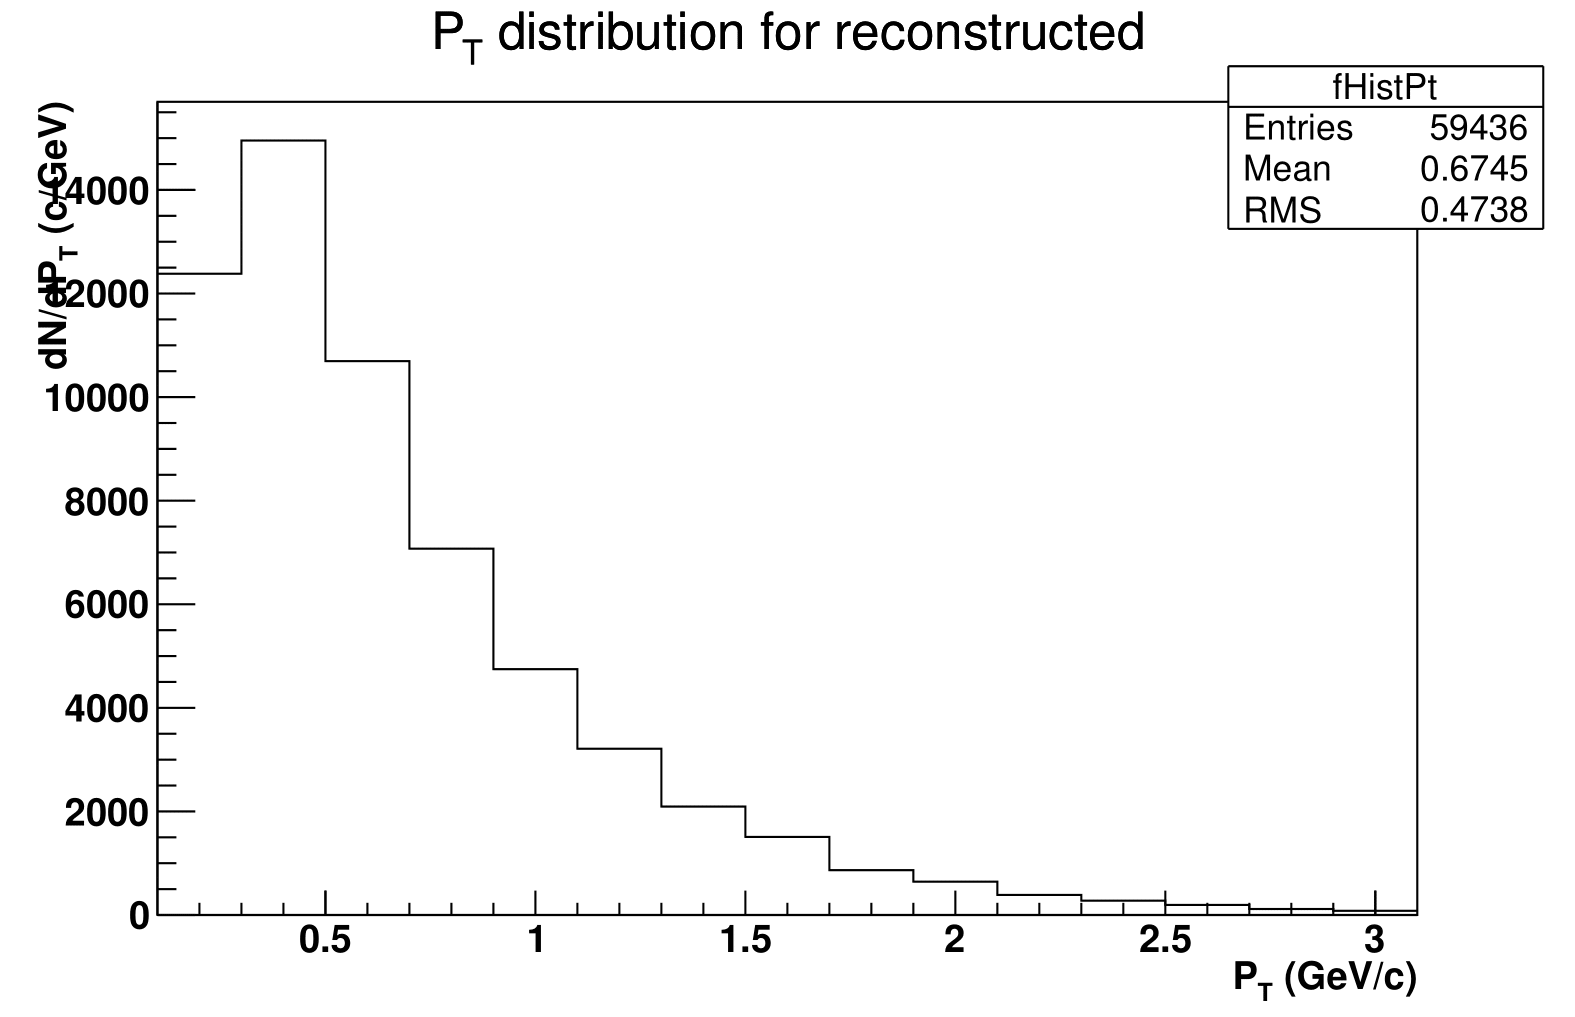
\includegraphics[width=1.0\textwidth]{figures/aliceplot_pt.png}
        \caption{Figure obtained from CERN Open Data platform, without any changes in the published code, using the Pb-Pb \href{http://opendata.cern.ch/record/1102}{data sample} at the collision energy of 2.76 TeV per nucleon pair from run number 139038.}
        \label{fig:alice_pt_distribution}
     \end{minipage}
\end{figure}

\subsection{LHCb Rare Charm Decay Search Example}
\vspace{-1em}
\textit{Struggles using Large Local Files and ROOT warnings}\\
Data analysis in experimental partile physics is notorious for the humongous amount of data that it handles. For most REANA examples, datasets are pulled from different (mostly online) sources, and are not uploaded directly using the \href{https://reana-client.readthedocs.io/en/latest/userguide.html}{reana-client upload file} option. Some use cases, however, require manual uploads of files by the researchers. 


\begin{figure}[H]
    \centering
    \begin{minipage}[H]{0.49\textwidth}
\noindent
\href{https://github.com/reanahub/reana-demo-lhcb-d2pimumu}{This LHCb example} studying the rare decay $D_{(s)}^{+}\rightarrow \pi^{+} \mu^{+} \mu ^{-}$ uses a 10 GB ROOT file. Debugging or changing parameters for different tests would then require uploading this large file at each run, which is redundant after the first upload in the REANA workspace. Hence, future work includes:
\begin{itemize}
    \item[i] allowing upload of files larger than the memory size by buffering technique.
    \item[ii] reusing the same file(s): REANA architecture could be restructured to use a shared workflow workspace, making debugging or iterative changes easier.
\end{itemize}

     \end{minipage}
 \hfill
    \begin{minipage}[H]{0.49\textwidth}
        \centering
        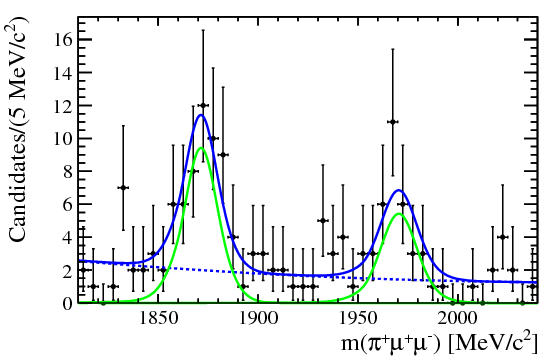
\includegraphics[width=1.0\textwidth]{figures/lhcb_eta.png}\\
        \caption{Centrality plot, obtained by running the analysis locally}
        \label{fig:lhcb_eta}
     \end{minipage}
\end{figure}
\noindent
Moreover, the ROOT analysis scripts would cause several warnings, although not leading to fatal errors. Nevertheless, such messages overflow the logging output and had to be cleaned. The \href{https://root-forum.cern.ch/}{ROOT forum} is a prime example of user support at CERN.


\subsection{ATLAS RECAST Example}
\vspace{-1em}
\textit{Dealing with Docker User Permissions}\\
One of the main technological advancements that allows now reproducibility of science are the \href{https://www.docker.com/}{docker images/containers}, which are isolated from one another and bundle their own software, libraries and configuration files. The \href{https://hub.docker.com/u/reanahub}{REANA docker images} are openly available online.

\begin{figure}[H]
    \centering
    \begin{minipage}[H]{0.49\textwidth}
This \href{http://www.reana.io}{REANA} reproducible analysis example demonstrates
a \href{https://indico.cern.ch/event/525142/contributions/2190137/attachments/1291681/1924055/RECAST-CAP-Reinterpretation-Workshop.pdf}{RECAST}\cite{recast-paper} analysis using \href{https://atlas.cern}{ATLAS} Analysis Software Group stack.

\vspace{1em}

\noindent
The user (e.g. researcher doing data analysis) only has to create a simple \href{https://github.com/reanahub/reana-demo-atlas-recast/blob/master/eventselection/Dockerfile}{Dockerfile} that mentions the required libraries for the execution of their code. One of their main features is that docker containers are more lightweight than virtual machines.

\vspace{1em}

\noindent
For \href{https://github.com/reanahub/reana-demo-atlas-recast}{this REANA example} for the \href{https://atlas.cern/}{ATLAS collaboration}, some files are in private workspaces not accessible by all users inside the docker container, hence the need to slightly change the original docker containers.
     \end{minipage}
 \hfill
    \begin{minipage}[H]{0.49\textwidth}
        \centering
        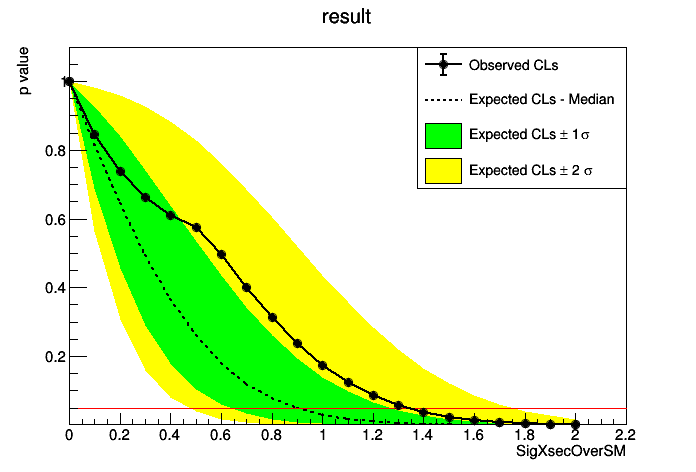
\includegraphics[width=1.0\textwidth]{figures/atlas_limit.png}\\
        \caption{Statistical analysis done via the RECAST method.}
        \label{fig:atlas_limit}
     \end{minipage}
\end{figure}



\begin{figure}[H]
    \centering
    \begin{minipage}[H]{0.49\textwidth}
\subsection{CMS Higgs to Four Leptons Decay}
\vspace{-0.25em}
\textit{Entrypoint scripts}\\
The discovery of the Higgs boson \cite{Higgs_discovery} created a lot of enthusiasm, and parts of this achievement have been reproduced inside REANA with \href{https://github.com/reanahub/reana-demo-cms-h4l}{this example}.\\
\vspace{1em}

\noindent
It studies the Higgs-to-four-lepton decay channel $H \to ZZ^{*} \to 4$ leptopns that led to the Higgs boson experimental discovery in 2012. The example uses CMS open data released in 2011 and 2012.\\
\vspace{1em}

\noindent
For convenience purposes, the \href{https://hub.docker.com/r/cmsopendata/cmssw_5_3_32}{CMSSW docker image} automatically sets the environment variables and aliases for the CMS user. When running the image through REANA though, the \href{https://github.com/clelange/cmssw-docker/blob/master/standalone/entrypoint.sh}{CMS entrypoint script} is overwritten and it has to be re-executed.

     \end{minipage}
 \hfill
    \begin{minipage}[H]{0.49\textwidth}
        \centering
        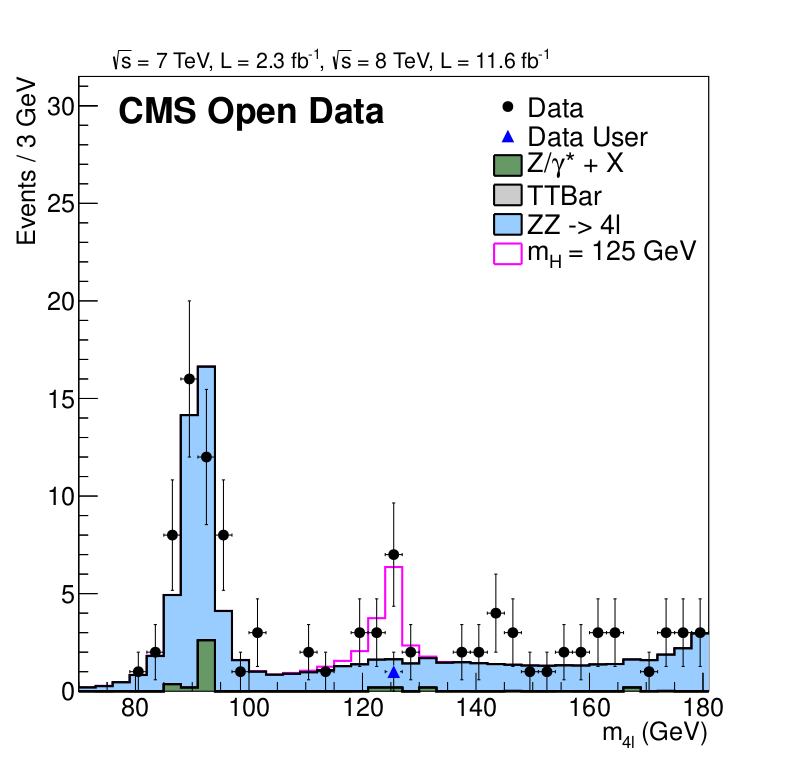
\includegraphics[width=1.0\textwidth]{figures/cms_h4l.png}\\
        \caption{Possible Higgs decay to four leptons.}
        \label{fig:cms_h4l}
     \end{minipage}
\end{figure}




\section{Workflow Factory for CMS AOD Reconstruction}
Some projects may have standardized/parametrized workflows, which only require some parameter changes for a different run, with small or no code changes. Such a project is the CMS reconstruction for \href{https://twiki.cern.ch/twiki/bin/view/CMSPublic/WorkBookDataFormats}{file formats}: from RAW to Analysis Object Data (AOD) files. For this purpose, we have designed a \href{https://github.com/reanahub/reana-demo-cms-reco}{workflow factory demo} that automatically creates the workflows based only on the selection of the dataset. 

\begin{figure}[H]
    \centering
    \begin{minipage}[H]{0.49\textwidth}
The workflow can be logically divided into two steps:
\begin{itemize}
    \item[i)] Polling information from the associated CERN Open Data page of the dataset
    \item[ii)] Change the template files using the polled information
\end{itemize}
\vspace{1em}
Three such workflows (for different years and datasets) have been manually created and tested, to be used as references for the workflow factory.

     \end{minipage}
 \hfill
    \begin{minipage}[H]{0.49\textwidth}
        \centering
        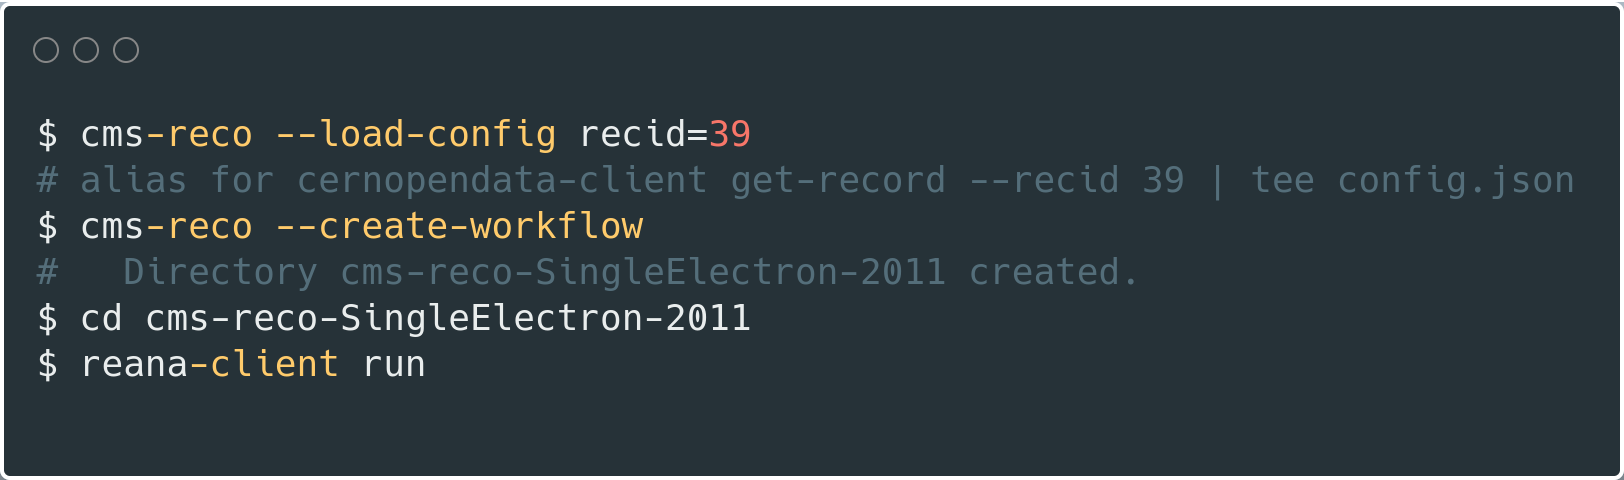
\includegraphics[width=1.0\textwidth]{figures/workflow_factory.png}
        \caption{Commands to create and execute a workflow using mostly default parameters for the dataset with record id 39, namely the SingleElectron 2011 \href{http://opendata.cern.ch/record/39}{dataset}.}
        \label{fig:workflow_factory}
     \end{minipage}
\end{figure}

\noindent
This significantly improves the user experience: before, one would have to manually extract all relevant information and create a reana.yaml file from scratch; but now, all the user has to do is install the package and run a simple (customizable) command. This paves the way for a more general workflow factory that could be used for arbitrary workflows.




\begin{figure}[H]
    \centering
    \begin{minipage}[H]{0.49\textwidth}
\section{Workflow Systems and Partial Workflow Execution}


The main and simplest workflow system is serial (built in-house), which REANA uses by default. However, more interesting examples benefit from more complicated workflow systems, which may have worthy features, e.g.  parallelism.

\vspace{1em}

\noindent
One regular task for REANA is to constantly update to the latest version of the respective workflow system, which may require API changes and other functionalities. Nevertheless, one feature that deemed important is the partial workflow execution, which implies that the user may specify how many and which steps of the workflow are actually executed. This proves itself important in debugging.

\vspace{1em}

\noindent
 As the CWL and YADGE have implemented this tool, it felt natural to include this feature for the serial workflow system as well.

     \end{minipage}
 \hfill
    \begin{minipage}[H]{0.49\textwidth}
        \centering
        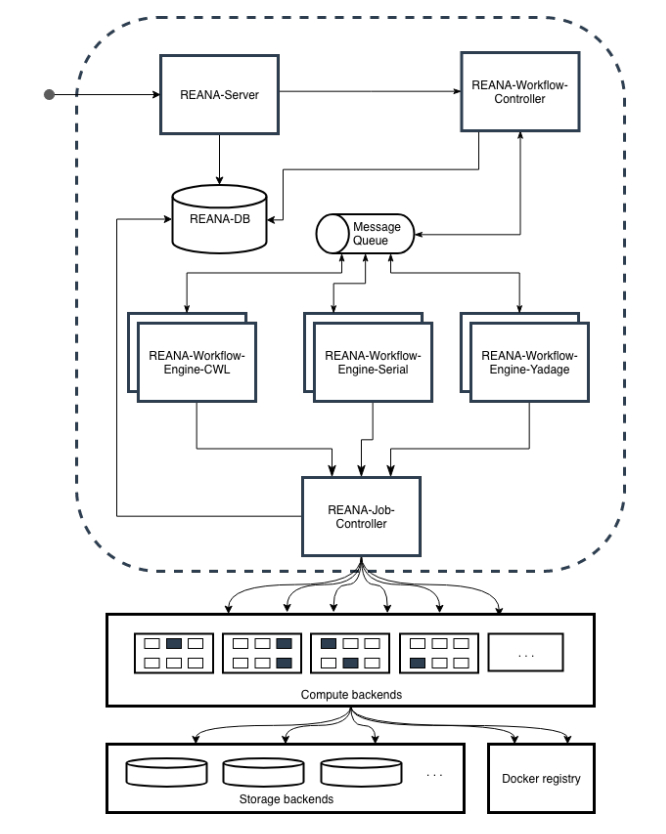
\includegraphics[width=1.0\textwidth]{figures/reana-stack.jpg}
        \caption{REANA cluster architecture and its components. Note the support for several workflow systems (CWL, Serial, Yadage). \cite{reana_paper}}
        \label{fig:reana-stack}
     \end{minipage}
\end{figure}


\section{Conclusion}
The aim of the REANA reproducible analysis platform is to provide modern information technology tools and solutions via a platform to scientists, such that they can structure their data analys in a reproducible, preservable, and shareable manner. This poses both technological and sociological challenges. On the technology side, one has to deal with large container sizes and massively parallel workflows. On the sociological side, one has to persuade researchers that adopting reproducibility best practices is not cumbersome, but it is actually helping their daily research.\\

\noindent
We have taken several typical examples from both data production and data analysis phases of the research conducted at CERN in order to study the feasibility and to demonstrate the applicability of the REANA approach. We hope that the advancement of technology through readily-applicable examples will help to drive the cultural change towards fair and open science.

\section*{Acknowledgements}
Over the past 13 weeks, I have received help and guidance from so many amazing people. Firstly, I would like to thank my supervisor, \href{https://orcid.org/0000-0001-7202-5803}{Dr. Tibor Šimko}, for his guidance and introducing me to this wonderful open science movement.

\noindent
I am proud to have been part of the \href{http://information-technology.web.cern.ch/about/organisation/digital-repositories}{IT-CDA-DR} department at CERN, working with the Open and Reproducible Research team: \href{https://orcid.org/0000-0003-0649-2002}{Diego Rodriguez Rodriguez}, \href{https://orcid.org/0000-0003-1064-6967}{Rokas Mačiulaitis}, \href{https://orcid.org/0000-0002-1416-3244}{Jan Okraska} and \href{https://orcid.org/0000-0003-4649-6630}{Leticia Wanderley}. Their help was the key to any progress in my project. Additionally, all the other members of the department were extremely friendly, helpful and informative.

\noindent
Secondly, thank you to \href{https://orcid.org/0000-0002-9803-6639}{Jean-Yves Le Meur} for selecting me and giving me so many projects to choose from for the best of my abilities.

\noindent
Additionally, thank you to the CERN Summer Student team, especially Adriana Bejaoui. It
has been the most incredible experience, and I am so grateful to have taken part in CERN.
